\subsection{Диффракция}

\begin{figure}[p]
	\centering
	\begin{subfigure}{\tw}
		\begin{tikzpicture}
			\begin{axis} [
				width			=	10cm,
				colormap 		= 	{GS}{rgb(0cm)=(.1, .1, .1)  rgb(1cm)	=	(1, 1, 1)},
				xlabel 			=	{$x$, $\frac{\lambda}{D}$},
				ylabel 			=	{$y$, $\frac{\lambda}{D}$},
				zlabel 			=	{$I/I_0$},
				ylabel shift 	= -.4 cm,
				xlabel shift 	= -.3 cm,
				ytick			= {-2,0,2},
				colorbar,
				colorbar style 	= {
				ytick 	= 	{0, .2, .4, .6, .8, 1.},
				}
				]
				
				\addplot3[
				samples				=	100,
				samples y			=	100,
				mesh,
				patch type			=	line,
				x filter/.code		=	\def\pgfmathresult{-5},
				smooth
				]
				table[x=x, y=y, z=I] {data/eiry-disk-x.txt};
				%
				\addplot3[
				samples			=	100,
				samples y		=	100,
				mesh,
				patch type		=	line,
				y filter/.code	=	\def\pgfmathresult{4.5},
				smooth
				]
				table[x=x, y=y, z=I] {data/eiry-disk-y.txt};
				
				\addplot3[surf] table[x=x, y=y, z=I] {data/eiry-disk.txt};
			\end{axis}
		\end{tikzpicture}
		\caption{}
		\label{}
	\end{subfigure}\\[2pc]
	\begin{subfigure}{\tw}
		\begin{tikzpicture}
			\begin{axis} [
				width			=	10cm,
				height			=	7.5cm,
				colormap 		= 	{GS}{rgb(0cm)=(.1, .1, .1)  rgb(1cm)	=	(1, 1, 1)},
				view			=	{0}{90},
				ytick 	= 	{-3, -2, ..., 3},
				colorbar,
				colorbar style 	= 	{
				ytick 	= 	{0, .2, .4, .6, .8, 1.},
				},
				xlabel 			=	{$x$, $\frac{\lambda}{D}$},
				ylabel 			=	{$y$, $\frac{\lambda}{D}$},
				]
				
				\addplot3[surf, shader=interp] table[x=x, y=y, z=I] {data/eiry-disk.txt};
			\end{axis}
		\end{tikzpicture}
		\caption{}
		\label{}
	\end{subfigure}
	\caption{}
\end{figure}

\begin{figure}[p]
	\centering
	\begin{subfigure}{\tw}
		\begin{tikzpicture}
			\begin{axis} [
				width			=	10cm,
				colormap 		= 	{GSW}{rgb(0cm)=(.1, .1, .1) rgb(.05cm)=(.99, .99, .99) rgb(1cm)	=	(1, 1, 1)},
				xlabel 			=	{$x$, $\frac{\lambda}{D}$},
				ylabel 			=	{$y$, $\frac{\lambda}{D}$},
				zlabel 			=	{$I/I_0$},
				ylabel shift 	= -.4 cm,
				xlabel shift 	= -.3 cm,
				ytick			= {-2,0,2},
				colorbar,
				colorbar style 	= {
				ytick 	= 	{0, .2, .4, .6, .8, 1.},
				}
				]
				
				\addplot3[
				samples				=	100,
				samples y			=	100,
				mesh,
				patch type			=	line,
				x filter/.code		=	\def\pgfmathresult{-5},
				smooth
				]
				table[x=x, y=y, z=I] {data/eiry-disk-x.txt};
				%
				\addplot3[
				samples			=	100,
				samples y		=	100,
				mesh,
				patch type		=	line,
				y filter/.code	=	\def\pgfmathresult{4.5},
				smooth
				]
				table[x=x, y=y, z=I] {data/eiry-disk-y.txt};
				
				\addplot3[surf] table[x=x, y=y, z=I] {data/eiry-disk.txt};
			\end{axis}
		\end{tikzpicture}
		\caption{}
		\label{}
	\end{subfigure}\\[2pc]
	\begin{subfigure}{\tw}
		\begin{tikzpicture}
			\begin{axis} [
				width			=	10cm,
				height			=	7.5cm,
				colormap 		= 	{GSW}{rgb(0cm)=(.1, .1, .1) rgb(.05cm)=(.99, .99, .99) rgb(1cm)	=	(1, 1, 1)},
				view			=	{0}{90},
				ytick 	= 	{-3, -2, ..., 3},
				colorbar,
				colorbar style 	= 	{
				ytick 	= 	{0, .2, .4, .6, .8, 1.},
				},
				xlabel 			=	{$x$, $\frac{\lambda}{D}$},
				ylabel 			=	{$y$, $\frac{\lambda}{D}$},
				]
				
				\addplot3[surf, shader=interp] table[x=x, y=y, z=I] {data/eiry-disk.txt};
			\end{axis}
		\end{tikzpicture}
		\caption{}
		\label{}
	\end{subfigure}
	\caption{}
\end{figure}

\begin{figure}[p]
	\begin{subfigure}[t]{\tw}
		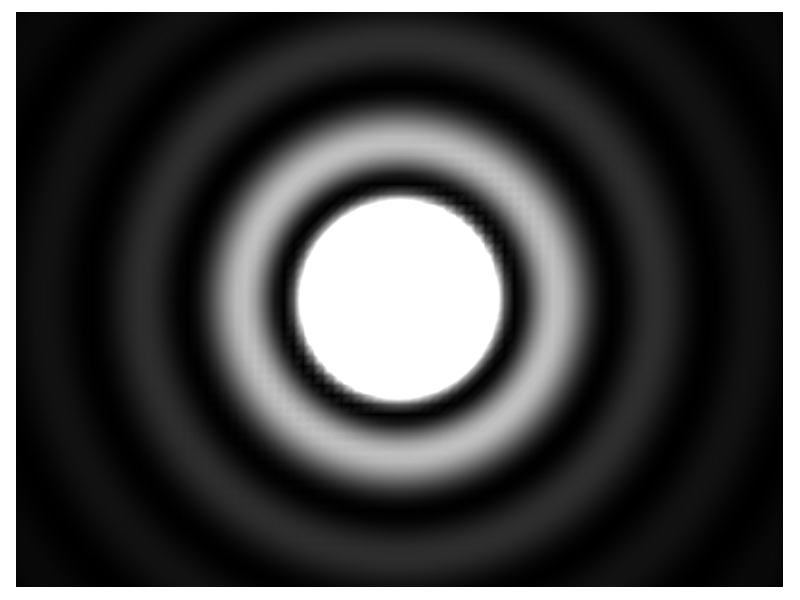
\includegraphics[width=4.7cm]{eiry-disk-0}\hfill
		\begin{tikzpicture}
			\begin{axis}[
				height	=	4.125cm,
				width	=	5.5cm,
				xlabel	=	{$x$, $\frac{\lambda}{D}$},
				ylabel	=	{$I/I_0$},
				ylabel shift	= -1 cm,
				]
				
				\addplot[smooth] table[x=x, y=e0]{data/eiry-disk-profile.txt};
			\end{axis}
		\end{tikzpicture}
		\caption{Диффракционное изображение от одного источника}
	\end{subfigure}\\
	\begin{subfigure}[t]{\tw}
		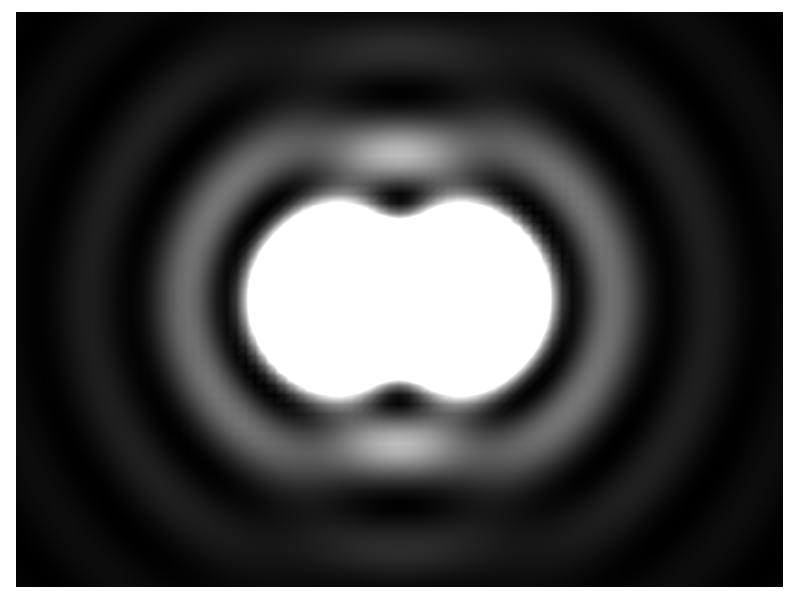
\includegraphics[width=4.7cm]{eiry-disk-1}\hfill
		\begin{tikzpicture}
			\begin{axis}[
				height	=	4.125cm,
				width	=	5.5cm,
				xlabel	=	{$x$, $\frac{\lambda}{D}$},
				ylabel	=	{$I/I_0$},
				ylabel shift	= -1 cm,
				]
				
				\addplot[smooth] table[x=x, y=e1]{data/eiry-disk-profile.txt};
			\end{axis}
		\end{tikzpicture}
		\caption{Диффракционное изображение от двух источников с разделением~$1.22\lambda/D$}
	\end{subfigure}\\
	\begin{subfigure}{\tw}
		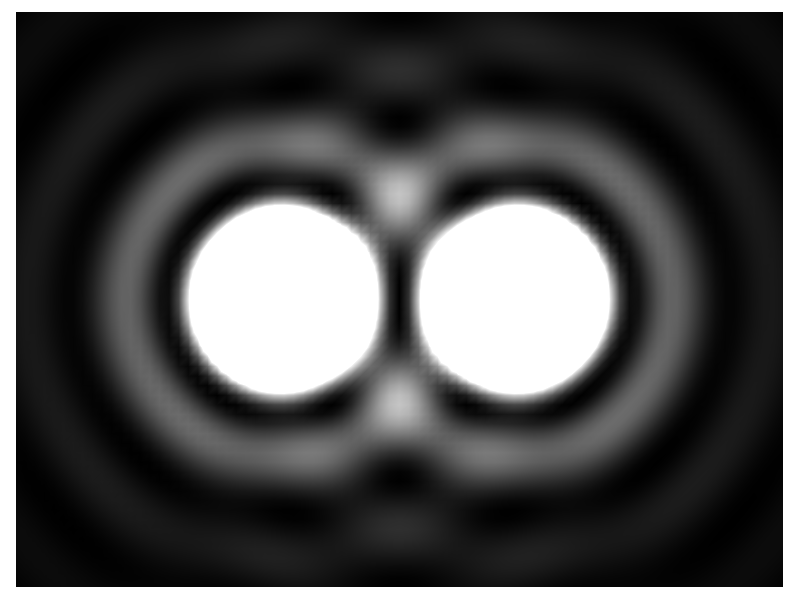
\includegraphics[width=4.7cm]{eiry-disk-2}\hfill
		\begin{tikzpicture}
			\begin{axis}[
				height	=	4.125cm,
				width	=	5.5cm,
				xlabel	=	{$x$, $\frac{\lambda}{D}$},
				ylabel	=	{$I/I_0$},
				ylabel shift	= -1 cm,
				]
				
				\addplot[smooth] table[x=x, y=e2]{data/eiry-disk-profile.txt};
			\end{axis}
		\end{tikzpicture}
		\caption{Диффракционное изображение от двух источников с разделением~$2 \cdot 1.22\lambda/D$}
	\end{subfigure}\\
	\begin{subfigure}{\tw}
		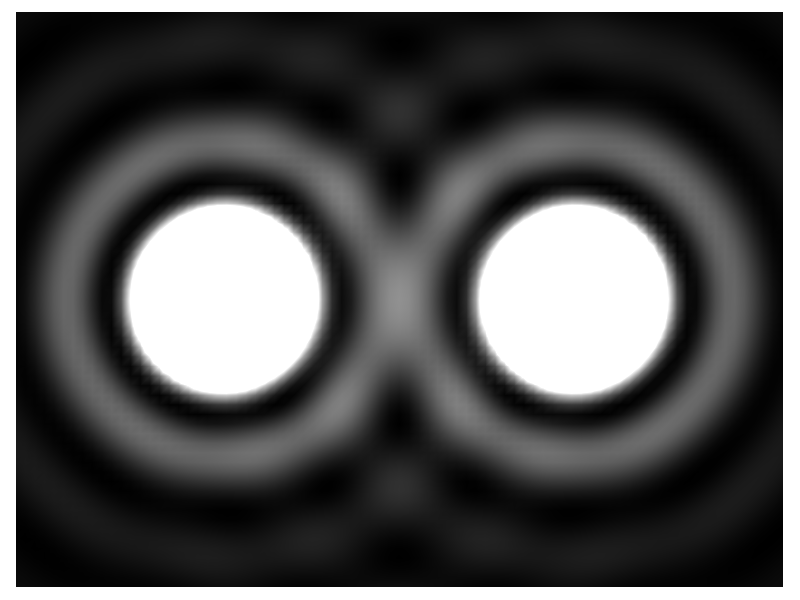
\includegraphics[width=4.7cm]{eiry-disk-3}\hfill
		\begin{tikzpicture}
			\begin{axis}[
				height	=	4.125cm,
				width	=	5.5cm,
				xlabel	=	{$x$, $\frac{\lambda}{D}$},
				ylabel	=	{$I/I_0$},
				ylabel shift	= -1 cm,
				]
				
				\addplot[smooth] table[x=x, y=e3]{data/eiry-disk-profile.txt};
			\end{axis}
		\end{tikzpicture}
		\caption{Диффракционное изображение от двух источников с разделением~$3 \cdot 1.22\lambda/D$}
	\end{subfigure}
	\caption{}
\end{figure}

